%\documentclass[letterpaper, paper,11pt]{AAS}
\documentclass[journal ]{new-aiaa}
\usepackage[utf8]{inputenc}
\usepackage{textcomp}
%\usepackage{amssymb}
\usepackage{amsmath}
\usepackage{graphicx}
%\usepackage{amsthm}
\usepackage[version=4]{mhchem}
\usepackage{siunitx}
\usepackage{longtable,tabularx}
\setlength\LTleft{0pt} 
%\newtheorem{theorem}{Theorem}
\newcommand{\state}{\ensuremath{\mathbf{x}}}
\newcommand{\control}{\ensuremath{\mathbf{u}}}
\newcommand{\ur}{\ensuremath{u_{\mathrm{ref}}}}
\newcommand{\State}{\ensuremath{\mathbf{X}}}
\newcommand{\Control}{\ensuremath{\mathbf{U}}}
%\newcommand{\costate}{\mathbf{p}}
%\newcommand{\multiplier}{\mathbf{\lambda}}
\newcommand{\param}{\ensuremath{\mathbf{p}}}
%\newcommand{\costate}{\mathbf{\lambda}}
%\newcommand{\multiplier}{\mathbf{\nu}}
\newcommand{\E}[1]{\mathbb{E}\left[#1\right]}
\newcommand{\V}[1]{\mathbb{V}[#1]}
\newcommand{\mean}{\mathbf{m}}
\newcommand{\cov}{C}
\newcommand{\std}{S}
\newcommand{\sample}{\ensuremath{\mathbf{z}}}
% Title Page
\title{Altitude-Optimal Mars Entry Guidance via Optimal Control Under Uncertainty}


\begin{document}
\author{Connor D. Noyes\thanks{Ph.D. Candidate, Department of Mechanical and Aerospace Engineering, University of California, Irvine, 92697} \ and Kenneth D. Mease\thanks{Professor Emeritus, Department of Mechanical and Aerospace Engineering, University of California, Irvine, 92697}}
\maketitle

% Refences with notes:
% AltitudeUnderUncertainty
% MarsEntryDesensitized % linearized but closed-loop with fixed gain. No consideration of saturation 
% EntryOUU % Does not use linearization, also doesnt solve in a conventional way, maybe remove?
% TrajectoryDesensitization % Desensitized like seywald and kumar, is it entry applied?
% EntryOUUThesis1 % Earth EDL, focuses on footprint computation, only considers open-loop in the reentry problem, and did not conduct monte carlo to confirm
% EntryOUUThesis2 % LQR, minimum control effort objective which stays away from the bounds, angle of attack as control variable. Does perform Monte Carlo(s) to validate improvement. 

%Rather than impose a chance constraint to reduce saturation, the control is freely allowed to saturate as long as the end result is good. 

% Ideas to discuss:
% Result of optimization is a reference trajectory and (linear) controller with desirable robustness 
% Demonstrate correlation between UT and MC results to validate use of the UT, but there are limits 
% Joint optimization (naturally) leads to superior results over fixed gains 
% Examine how solutions change with weights, and also initial state vs parametric uncertainty 
% Conclusions? New approach to combined reference + controller design 

\section*{Abstract}
%The current generation of Mars entry vehicles employ a modified Apollo entry guidance that performs range control until a fixed velocity, and key trajectory metrics are the total range error and altitude at parachute deploy. We pose the entry guidance problem as an optimal control problem under uncertainty with closed-loop dynamics to determine a reference trajectory that is optimal with respect to an objective that weights mean altitude, altitude variance, and distance variance. The result is a reference trajectory with optimal margin for a given set of input dispersions. The robustness and optimality are validated in a Monte Carlo analysis. Novel aspects of the approach include use of the unscented transform to account for saturation in the closed-loop system, and the use of differential dynamic programming to solve the challenging nonlinear optimal control problem. 
\section*{Introduction}
\lettrine{A}{ltitude} maximization is of interest to both current and next generation Mars missions. Maximizing altitude at chute deployment allows for landing at higher elevations, which are motivated by reasons of scientific interest, as well as for increasing timeline margin for subsequent descent and landing operations in high ballistic coefficient vehicles.
Future missions, including sample return \cite{MSR} and manned missions, will place even greater emphasis on robustness and performance than the current generation, such as a pinpoint landing requirements \cite{EvolvableMars}. The guidance design methodology used on the latest Mars entry vehicles is to first design a reference trajectory that satisfies mission requirements and constraints, and potentially optimizes a performance index as well. Then, a controller is chosen and tuned until the performance is satisfactory. Mar Science Laboratory and Mars 2020 both chose the entry terminal point controller \cite{MSL_EDL,M2020_EDL}, a modified version of the Apollo second phase guidance \cite{MSL_EDL2}. Because the controller gains are derived from the reference trajectory, proper design of the reference is the most important part of the guidance design. If the necessary performance cannot be achieved through tuning, the reference trajectory is changed and the process is repeated.

In this work we propose an approach to entry guidance based on optimal control under uncertainty that performs trajectory optimization with knowledge of the controller design and uncertainties affecting the problem. This approach blends optimal control, specifically altitude maximization, with uncertainty quantification to incorporate statistical uncertainty in the vehicle initial state and model parameters, such as ballistic coefficient or atmospheric density. By formulating the uncertain optimal control problem in a closed-loop setting, more robust performance can be achieved than by conventional design methods.

\subsection*{Related Work}
\subsubsection*{Altitude Maximization}
The motivation behind altitude maximization in Mars entry is to provide sufficient timeline for subsequent descent and landing operations. The problem of maximizing the terminal altitude of Mars entry vehicles has been studied in a deterministic setting
\cite{AltitudeOptimization} % this one "proves" the switch numbers 
\cite{AltitudeOptimizationIndirect}
\cite{GuangfeiDissertation}
and also in a stochastic setting \cite{AltitudeUnderUncertainty} where linear covariance techniques were used to reduce open-loop covariance, and in \cite{MarsEntryDesensitized} sensitivity terms related to variations in the initial state are considered.

\subsubsection*{Optimal Control with Sensitivity/Covariance Reduction}
The literature on optimal control problems that weight a nominal optimization objective with covariance or sensitivity terms is vast, and the idea has seen a large amount of attention within the entry guidance community including \cite{AltitudeUnderUncertainty, MarsEntryDesensitized, EntryOUUThesis1, EntryOUUThesis2, EntryOUU}.
The focus has been on making open-loop trajectories more robust, regardless of whether the loop will be closed for the real system. This focus on open-loop strategies is one reason why the issue of control saturation has not been adequately addressed. An additional reason is the (nominal) optimization objective under consideration: altitude optimal trajectories are known to be bang-bang \cite{AltitudeOptimization} while other objectives such as maximum crossrange trajectories, studied in \cite{EntryOUUThesis2}, are not.  

One common feature of these studies is the use linear propagation techniques to compute sensitivity matrices or covariance matrices, which we will demonstrate is insufficient for closed-loop optimization in the presence of control saturation. Our use of the unscented transform allows us to accurately capture the effects of saturation on performance. Although the unscented transform has been used in the context of optimal control under uncertainty \cite{UnscentedOptimalControl}, the focus remained on open-loop strategies. 

While a number of these reports note the possibility of closed-loop covariance reduction, only \cite{MarsEntryDesensitized}, where the linear approach to uncertainty quantification is used with a fixed gain matrix, and \cite{EntryOUUThesis2}, where the Linear Quadratic Regulator (LQR) approach is used, actually examine this scenario, and both apply the linear approach to uncertainty quantification.

\subsubsection*{Differential Dynamic Programming}
Differential dynamic programming (DDP) \cite{DDP} is a shooting method originally devised to solve unconstrained nonlinear optimal control problems that has since seen numerous extensions, including to constrained problems \cite{DDP_ControlLimited,HDDP1,HDDP2,DDP_NonlinearConstraints,DDP_InteriorPoint}, and stochastic problems \cite{iLQG, DDP_Stochastic, ozaki_UT,ozaki2020tube}. 

A common theme among all of these references is their application to robotics \cite{iLQG, DDP_Stochastic} or low thrust trajectory optimization \cite{HDDP1,HDDP2,ozaki_UT,ozaki2020tube}. Despite the apparent success in these fields, DDP has not yet garnered much attention in the entry guidance community. Simultaneous transcription methods, especially collocation methods, are popular for their ability to readily handle nonlinear constraints on states and controls, and indeed for deterministic problems with low state dimension, their applicability and effectiveness is undeniable. In a stochastic setting, however, the most common methods of converting the problem to a deterministic one involve an increase in the dimensionality of the state vector that render the problem difficult to solve this way.

\subsection*{Contributions}
The entry guidance problem is posed as an uncertain optimal control problem with a mean-variance objective. The dynamics are in a closed-loop formulation that allows for arbitrary feedback laws to be used. Use of samples, in particular the unscented transform, addresses the issue of control saturation - a key issue in Mars entry guidance that has not been discussed in the context of variance reduction except in the fuel-optimal powered descent problem \cite{DesensitizeFuelOptimal}. A unifying theme of the previous literature is the use of linear covariance techniques, which we argue are insufficient for the problem at hand. 

As a second contribution, we demonstrate that differential dynamic programming is a natural choice for solving the nonlinear optimal control problem because the method scales favorably compared to the collocation methods utilized in  other covariance reduction methods. Despite its popularity in robotics and low thrust trajectory applications, DDP has seen virtually no use in entry trajectory optimization. 

More concretely, consider an optimal control problem in which the system is described by $n$ states, $m$ controls, and discretization of the independent variable into $N$ stages. In an uncertain setting, the most common ways to incorporate distribution information involve including $n\times n$ sensitivity terms, or $\frac{n(n+1)}{2}$ covariance terms, or use sample-based approximations in which the state dimension with $S$ samples yields state dimension $Sn$. This increased state dimension poses fewer problems in DDP, which iteratively solves $N$ optimization problems in $m$ variables, compared to direct methods, which solve a single large scale problem in $N(n+m)$ variables.

%In entry guidance problems, performance is characterized by extrema of one or more quantities of interest, e.g. trajectories with low altitude or high Mach number at parachute deployment. Altitude optimal trajectories are bang-bang in nature, and leave no margin for feedback control. The amount of margin that ought to be left is a function of the system uncertainty and the guidance algorithm chosen to correct off nominal performance. Clearly, then, for a fixed uncertainty set and guidance algorithm, there exists an optimal tradeoff between mean performance, and tail performance of closed-loop cases. Our goal is to compute such an optimal reference trajectory and margin. 


%One way to characterize the distribution of a quantity is with its mean and variance, which motivates propagation of these moments as an efficient alternative to propagating the entire distribution. The most efficient method is linear propagation; for linear systems with Gaussian distributed uncertainty the result is exact, but for nonlinear systems the method can be inaccurate. The unscented transform is a sampling-based method that propagates a set of sigma points through the nonlinear dynamics and reconstructs the mean and covariance from the transformed samples.

%Typical trajectory optimization designs a reference trajectory that can be utilized in different ways to achieve the guidance objective. However, the optimality of this reference trajectory is directly at odds with robust closed-loop performance for several problems of interest in entry guidance: altitude maximization and propellant minimization.  

%\section{Terminology: Uncertain vs Stochastic}
% Stochastic optimal control is concerned with systems governed by stochastic differential equations
% \begin{align*}
% \mathrm{d}\state = f(t,\state)\mathrm{d}t + g(t,\state)\mathrm{d}w
% \end{align*}
% where $w$ is a Standard Brownian motion and the initial state may be given by a distribution or a single state. The problem is subject to the rules of stochastic calculus and the partial differential equation (PDE) governing the evolution of the probability density of the state vector is the Fokker-Planck equation. 
% 
% In contrast, uncertain optimal control concerns systems governed by ordinary differential equations with initial conditions governed by a distribution, and the PDE that governs the probability density evolution is the Liouville equation.

%In both types of problems, the objective function is expressed probabilistically, often via expectations and variances, and constraints are incorporated as chance constraints. 

%The distinction has the following impact on SDDP algorithm: all terms related to diffusion term vanish, and the forward/backward simulations are conducted without noise. In Ozaki's approach, the backward pass computes expectations of the derivative terms. In constrast, we compute deterministic derivatives with respect to the extended state vector, and only compute the expectations in the cost function. 

%\section{Optimal closed-loop Trajectory Planning Under Uncertainty}
%The nonlinear dynamics are assumed to be affine in the control variable(s), which are saturated, and the initial state is assumed to be normally distributed
%\begin{align}
%\dot{\state} = p(\state) + q(\state)\mathrm{sat}(\control) ,\;
%\state(t_0)\sim N(\state_0,\,P_0)
%\end{align}
%Despite the nonlinear dynamics, it is assumed the state distribution remains well described by its first two moments, and thus we define 
%\begin{align}
%\mean &= \E{\state},\;\mean(t_0) = x_0 \\
%\cov &= \V{\state},\;\cov(t_0) = \cov_0
%\end{align}
%The objective is to determine a nominal control history $\control(t)$ that will steer the mean state to a terminal manifold $\psi(\mean(t_f)) = 0$ while minimizing the terminal cost $\phi(\mean(t_f), \cov(t_f))$. Adjoining the constraint to the cost with a vector of Lagrange multipliers yields
%\begin{align}
%J = \phi + \nu^T\psi
%\end{align}
%
%
%In our approach, samples are propagated through the full nonlinear dynamics, and the moments are computed from a finite set of samples $\sample_i,\,i=1,...,N$:
%\begin{align}
%\mean &\approx N^{-1}\sum_{i=1}^{N} \sample_i \\
%\cov &\approx N^{-1}\sum_{i=1}^{N} (\sample_i-\mean)(\sample_i-\mean)^T
%\end{align}

\section*{Closed-Loop Altitude-Optimal Entry Trajectory Design}
The problem of designing a robust entry reference trajectory is posed an optimal control problem under uncertainty. Following the approach taken by MSL and M2020, only the longitudinal motion is accounted for in the reference trajectory design; a separate lateral guidance logic determines when bank reversals should be commanded to prevent large crossrange distances to the target.
The longitudinal equations of motion of a point-mass model of a Mars entry vehicle are written with respect to the planet-relative vehicle velocity magnitude, and the state vector $\state$ consists of the vehicle altitude about the surface, the flight path angle, and the downrange distance flown. The control is the cosine of the bank angle, and thus the dynamics may be written
\begin{align}
h' &= \frac{v\sin\gamma}{-D - g\sin\gamma} \label{eq_dynamics_altitude}\\
s' &= \frac{v\cos\gamma}{-D - g\sin\gamma} \\
\gamma' &= \frac{\frac{L}{V}u + \left(\frac{v}{h+r_p}-\frac{g}{v}\right)\cos\gamma}{-D - g\sin\gamma} \label{eq_dynamics_fpa}
\end{align}
where $r_p$ is the planet radius, $g=\mu/(h+r_p)^2$ is the magnitude of the gravitational acceleration, and the lift and drag accelerations are
\begin{align}
D = \frac{1}{2}\frac{\rho}{\beta} v^2 \\
L = D(\frac{L}{D})
\end{align}
where $\rho=\rho_0\exp\left(-\frac{h}{h_s}\right)$ is an exponential model of the atmospheric density, $\beta=\frac{m}{C_DS}$ is the ballistic coefficient, $m$ is the vehicle mass, and $L/D$ is the lift-to-drag ratio.
The initial state vector is assumed to be governed by a distribution with first two moments $\E{\state(v_0)} = \state_0$, $\V{\state(v_0)} = \cov_0$. In this work, we assume the initial state is distributed according to $\state(v_0)\sim N(\state_0,\,\cov_0)$, but the assumption of normality is not required.
The guidance law is assumed to be to a saturated linear state feedback 
\begin{align}
u(v,\state) &= \mathrm{sat}_{[0,1]}\left(\ur(v) + \delta u(\state)\right)\\
\delta u &= k_D\delta D + k_{\gamma}\delta\gamma + k_s\delta s
\end{align}
where we note that, consistent with state-of-the-art EDL operations on Mars, drag acceleration has been used as a feedback term in place of altitude. The gains $k_i$ may be functions of velocity, and the saturation function is defined
\begin{align*}
\mathrm{sat}_{[a,b]}(x) = \left\{\begin{array}{lc}
        a, &  x < a\\
        x, &  a\le x \le b\\
        b, &  b < x
        \end{array} \right. % The period stops a warning about not closing the left 
\end{align*}
The saturation function is required to ensure that regardless of the value of the reference control \ur, the closed-loop control $u(v,\state)$ always satisfies the control limits. 
%Two scenarios will be considered. In the first, only the open-loop control $u_0$ is determined by the optimal control solution; the feedback gains are not included as optimization variables, but may still be functions of the planned trajectory, as in e.g. Apollo guidance, which computes influence coefficients around a nominal trajectory. In this setting, DDP searches for the most robust path subject to a given guidance approach. In the second scenario, the gains are included as controls to be determined via DDP. 

The objective is to determine the piece-wise constant reference control $\ur\left[v_0,v_f\right]$ that optimizes the altitude at chute deployment, which occurs at a fixed terminal velocity $v_f$. The weight $w_h$ allows for additional emphasis on the low end of the distribution. Additionally, while the mean downrange distance is unconstrained, there is a penalty on standard deviation of the downrange distance. For small weights $w_s$, this term is used to discourage solutions from sacrificing downrange accuracy for small altitude improvements. Larger weights encourage greater reduction in downrange errors at the expense of altitude.  There are no terminal constraints, and thus the optimal control problem is to minimize the objective functional
\begin{align}
%J &= -\E{h(v_f)} + w_h\V{h(v_f)}^{\frac{1}{2}} + w_s\V{s(v_f)}^{\frac{1}{2}}.
J(\ur) &= -\E{h(v_f)} + w_h\sigma_h(v_f) + w_s\sigma_s(v_f) \label{eq_objective}
\end{align}
subject to the equations of motion $\ref{eq_dynamics_altitude}-\ref{eq_dynamics_fpa}$, the initial conditions $\E{\state(v_0)} = \state_0$, $\V{\state(v_0)} = \cov_0$, and the bounded control $0 \le \ur(v) \le 1$.

\subsubsection*{Remark} Either variances or standard deviations may be used in the objective function. In practice, appropriate choices of the weights can produce equivalent results, but standard deviations are preferred because they are in the same units as the state variables, and allow for more natural interpretations of the weights. One consideration is that the square root is not differentiable at zero, but both in theory and in practice the terminal standard deviations are never exactly zero since the covariance matrix is positive definite.
\subsubsection*{Remark} Uncertainty in the parameters in governing differential equations can be included by appending the state vector with the parameters $\param$ with trivial dynamics $\dot{\param}=\bf0$.

%In summary, the optimal control problem under consideration is 
%	\begin{align}
%	\min_{\ur\left[v_0,v_f\right]}\ J\\  % 
%	\mathrm{subject\,to\,} \nonumber\\ 
%	&\mathbf{\state'} = f(v,\state,\ur) \\
%	&\E{\state(v_0)} = \state_0 \\
%	&\V{\state(v_0)} = \cov_0 \\
%	&0 \le \ur(v) \le 1 
%	\end{align}

\section*{Solution via Unscented Transform and DDP}
In order to compute the expected value and standard deviations in the objective function, the unscented transform \cite{UT1997} is used. This results in a deterministic problem with an extended state vector. The unscented transform is preferable to linear covariance techniques because the sigma points are propagated through the nonlinear, saturated dynamics, and are thus able to capture these effects more accurately than linearization. It is also preferable to random sampling because the number of sigma points is generally lower than the number of samples required for equivalent precision. %TODO: citation?

Next, because control saturation is a key issue in the closed-loop dynamics, the control-limited box-DDP algorithm \cite{DDP_ControlLimited} is employed to solve for the control updates during the backward pass. While this approach results in reference controls that satisfy the control limits, the saturation function is required in the forward pass to ensure the closed-loop sigma point trajectories also respect the control limits, or the predicted covariance will be underestimated.

\subsection*{Unscented Transform}
The unscented transform is a method to approximate the first two moments of a nonlinear transformation of a probability distribution. Consider a scalar quantity $q\in\mathbb{R}$ given by a nonlinear transformation $q = F(\param)$ of a vector $\param\in\mathbb{R}^n$ with known mean and covariance
\begin{align*}
\E{\param} &= \bar{\param}\\
\V{\param} &= \cov_{\param}.
\end{align*}
A set of $2n+1$ sigma points and associated weights are computed 
\begin{align*}
\param_0 &= \bar{\param} \\
\param_i &=  \bar{\param} + \left(\sqrt{\beta \cov_{\param}}\right)_i \\
\param_{i+n} &=  \bar{\param} - \left(\sqrt{\beta\cov_{\param}}\right)_i \\
w_0 &= \frac{\beta - n}{\beta} \\
w_i &= w_{i+n} = \frac{1}{2\beta}
\end{align*}
where $\beta$ is a scaling parameter, and $\left(\sqrt{\beta \cov_{\param}}\right)_i$ is the $i^{\mathrm{th}}$ column of the matrix square root of $\beta P_{\param}$. The sigma points are then mapped through the transformation
\begin{align}
q_i = F(\param_i),\;\;i=0,...,2n
\end{align}
and finally, the mean and variance are approximated using the weights and transformed sigma points
\begin{align*}
\E{q} &\approx \sum_{i=0}^{2n}w_iq_i  \triangleq \bar{q}\\
\V{q} &\approx \sum_{i=0}^{2n}w_i\left(q_i - \bar{q}\right)^2
\end{align*}

\subsection*{Control-Limited Differential Dynamic Programming}
In this section we review the differential dynamic programming method that will be used to solve the optimal control problem. 
The algorithm is formulated in discrete time, so the continuous time dynamics are discretized using Euler integration:
\begin{align}
\state_{i+1} = f(v, \state_i,\control_i) = \state_i + \state_i'\Delta v \label{eq_discrete_dynamics}
\end{align}
A trajectory $\{\State,\Control\}$ is a sequence of controls $ \Control=\{\control_0,\control_1,...,\control_{N-1}\} $ and corresponding states $\State=\{\state_0,\state_1,...,\state_N\}$ determined by integrating (\ref{eq_discrete_dynamics}) from $\state_0$.
Although the optimal control objective as posed considers only a terminal cost, in this section we consider a generic cost function $J$ consisting of a sum of running costs $l$ and a terminal cost $l_N$:
\begin{align}
J(\state_0,\Control) = \sum_{i=0}^{N-1}l(\state_i,\control_i) + l_N(\state_N)
\end{align}
Let $\Control_i$ be the tail of the control sequence, $\{\control_i,\control_{i+1},...,\control_{N-1}\}$, and the cost-to-go $J_i$, defined as the partial sum of costs from $i$ to $N$ is
\begin{align}
J_i(\state,\Control_i) = \sum_{j=i}^{N-1}l(\state_j,\control_j) + l_N(\state_N)
\end{align}
The Value function at timestep $i$ is the optimal cost-to-go at \state
\begin{align}
V_i(\state) = \min_{\Control_i} J(\state, \Control_i)
\end{align}
and at the final timestep the Value function is equal to the terminal objective. The Dynamic Programming principle reduces the problem of minimization over $\Control_i$ to a sequence of minimizations over $u$ at each timestep 
\begin{align}
V(\state) = \min_{\control}\left[l(\state,\control) + V^+(f(\state,\control))\right] \label{eq_dynamic_programming}
\end{align}
where $V^+$ is the Value at the next time step.
Let the pseudo-Hamiltonian $Q(\delta\state,\delta\control)$ be the change in Value function as a function of perturbations to the pair $(\state,\control)$:
\begin{align}
Q(\delta\state,\delta\control) = l(\state+\delta\state,\control+\delta\control) + V^+(f(\state+\delta\state,\control+\delta\control))
\end{align}
The second order expansion of $ Q $ is given by
\begin{align}
Q_\state &= l_\state + f_\state^T V^+_\state \\
Q_\control &= l_\control + f_\control^T V^+_\state \\
Q_{\state\state} &= l_{\state\state} + f_\state^T V^+_{\state\state}f_\state + V^+_\state f_{\state\state} \\
Q_{\control\state} &= l_{\control\state} + f_\control^T V^+_{\state\state}f_\state + V^+_\state f_{\control\state} \\
Q_{\control\control} &= l_{\control\control} + f_\control^T V^+_{\state\state}f_\control + V^+_\state f_{\control\control}
\end{align}
where the subscripts denote partial derivatives with respect to that quantity, and the final term in each of the Hessians are tensor-vector contractions.
\subsubsection*{Remark} The terms $f_{\state\state},\, f_{\state\control}$ are $n\times n\times n$ and $n\times n\times m$ tensors, respectively, that must either be stored at $N$ timesteps, or else recomputed in the event the backward pass must be repeated with increased regularization. For large $n$, both computing and storing these quantities is problematic. Unfortunately, removing these terms entirely, as is done in the iterative Linear Quadratic Gaussian method \cite{iLQG}, leads to poor performance for the problem under consideration. In particular, the first order algorithm has a noticeably smaller radius of convergence, and different guesses at the initial control sequence often lead to different local minima. In contrast, the full second order DDP algorithm consistently converges to a single minimum from most guesses. Thus, we propose a compromise in which only the $n\times m \times m$ tensor $f_{\control\control}$ is retained in the above equations. Numerical experiments suggest this is sufficient to avoid poor solutions, at the expense of a slower convergence rate than the full algorithm with all second order terms included. However, in the situation at hand, in which the number of controls $m$ is fixed and small ($ \le4 $), and the state dimension, which depends on the number of uncertainties under consideration, is large ($20 < n <60$) this modification proves to be enabling for $n\ge 30$ with $N=1000$. A limited memory version of the Quasi-Newton approximations to these terms proposed in \cite{QNDDP} may also be a good choice to obtain superlinear convergence properties of the approximated second order algorithm while reducing the memory required. 
%(This reduces complexity from cubic in $n$ to linear)

The optimal control modification $\delta\control^*$ for some perturbation $\delta\state$ is a locally-linear feedback control $\delta\control^* = \mathbf{k} + K\delta\state$ obtained by minimizing the quadratic model subject to linear bounds on the controls
\begin{align}
\mathbf{k} = &\arg\min_{\delta\control} Q(\delta\state,\delta\control) \\
&\mathrm{subject\,to\,\;} \nonumber\\
\control_{\min}\le&\control+\delta\control \le\control_{\max}
\end{align}
and $K = -Q_{\control\control}^{-1}Q_{\control\state}$. Substituting the optimal control into the expansion of $Q$, a quadratic model of $V$ is obtained with derivatives
\begin{align}
\begin{split}
\label{eq_value_recurse}
V_\state &= Q_{\state}- K^TQ_{\control\control}\mathbf{k}\\
V_{\state\state} &= Q_{\state\state} - K^TQ_{\control\control}K.
\end{split}
\end{align}
The backward pass is performed by initializing $V$ and its derivatives with the value and derivatives of the terminal objective, then recursively computing the optimal control policy and (\ref{eq_value_recurse}).

The forward pass uses the newly computed control policy to integrate the new trajectory, subject to a backtracking line search
\begin{align}
\hat{\state}_0 &= \state_0 \\
\hat{\control}_{i} &= \control_i + \alpha \mathbf{k}_i + K_i(\hat{\state}_i - \state_i)\\
\hat{\state}_0 &= f(\hat{\state}_i,\hat{\control}_i)
\end{align}
where parameter $\alpha$ is a search parameter initialized to 1 and reduced until the Value function shows improvement. The backward-forward iterations are repeated until convergence to a locally optimal trajectory.

\subsection*{Objective Reformulation}
In order for DDP to be applied to this problem for arbitrary $w_h,w_s\ge 0$, it is essential to reformulate some or all of the objective terms as running costs rather than terminal costs. This is because the terminal formulation results in singularity of the Hessian of the pseudo-Hamiltonian with respect to the control, and this quantity must be invertible for the algorithm to proceed. In practice, one could also add a small control regularization term to the objective, but experience has shown that reformulating the mean altitude objective is sufficient. Due to linearity of the expectation operator, we have the following relationships for the time rate of change of the first two moments
\begin{align}
\frac{d }{d t}\E{x} &= \E{\dot{x}} \\
\frac{d }{d t}\V{x} &= \E{2x\dot{x}} - 2\E{x}\E{\dot{x}} \\
\sigma_x &= \V{x}^{\frac{1}{2}} \\
\frac{d }{d t}\sigma_x &= \frac{1}{2\sigma_x}\frac{d }{d t}\V{x}
%\frac{d }{d t}\V{x}^{\frac{1}{2}} &= \frac{1}{2\V{x}^{\frac{1}{2}}}\frac{d }{d t}\V{x}
\end{align}
and thus running cost used in the reformulated objective function is 
\begin{align}
%J = \int_{v_0}^{v_f}-\E{h'} +  2w_h(\E{hh'}-\E{h}\E{h'}) + 2w_s(\E{ss'}-\E{s}\E{s'})\mathrm{d}v \\
%J = \sum_{i=0}^{N-1} \left[-\E{h'} +  2w_h(\E{hh'}-\E{h}\E{h'}) + 2w_s(\E{ss'}-\E{s}\E{s'})\right]\delta v 
l(\state,\control) = -\E{h'} +  2w_h(\E{hh'}-\E{h}\E{h'}) + 2w_s(\E{ss'}-\E{s}\E{s'})
\end{align}
where $(\cdot)' = \frac{\dot{(\cdot)}}{\dot{v}}$.

\subsubsection*{Remark} While reformulating the mean altitude objective is essential to solving the problem, especially when $w_s=w_h=0$, reformulating the standard deviation terms is not. However, in numerical experiments we found that while both formulations result in the same solution, using running costs for the standard deviations allows DDP to converge in noticeably fewer iterations.

The non-differentiability of the saturation function in the controller also produces difficulties for the DDP algorithm, and thus we substitute the following smooth approximation when solving the optimal control problem
\begin{align*}
\mathrm{sat}_{[0,1]}(x) \approx \frac{1}{2} + \frac{1}{4K}\log\left(\frac{\cosh (2Kx)}{\cosh (2K(x-1))}\right) 
\end{align*}
where $K$ is a tuning parameter. $K=20$ in our implementation.

%\section*{Uncertainty Quantification}
%Show that in the presence of saturation and with a closed-loop, linearization isn't appropriate. 
%
%\begin{table}[h]
%%\caption{Comparison between uncertainty quantification methods for open-loop simulations. Both the linear propagation and the unscented transform are quite close the Monte Carlo values.
%\begin{tabular}{|c||c|c|}
%\hline
%UQ Method & $3\sigma$ Low Altitude & $3\sigma$ Range Error \\
%\hline
%Linear & 6.744 & 66.510 \\
%%\hline
%%Saturated Linear & 6.744 & 66.510 \\
%\hline
%Unscented Transform & 6.627 & 66.980 \\
%\hline
%Monte Carlo & 6.588 & 66.696 \\
%\hline
%\end{tabular}
%
%\end{table}
%\begin{table}[h]
%\begin{tabular}{|c||c|c|}
%\hline
%UQ Method & $3\sigma$ Low Altitude & $3\sigma$ Range Error \\
%\hline
%Linear & 5.678 & 4.453 \\
%%\hline
%%Saturated Linear & 5.877 & 4.543 \\
%\hline
%Unscented Transform & 4.876 & 8.854 \\
%\hline
%Monte Carlo & 4.817 & 8.168 \\
%\hline
%\end{tabular}
%\end{table}
%\begin{table}[h]
%    \begin{tabular} {|c|c||>{\centering}p{.9cm}|>{\centering}p{.9cm}|>{\centering}p{.9cm}|c|}
%        \hline
%        $Truth$ & $Predicted$ & ADA & SVM & GLM & Blended \\ \hline
%        T & T & 512 & 463 & 423 & 472 \\ 
%        T & F & 19  & 68  & 108 & 0   \\ 
%        F & T & 5   & 85  & 67  & 22  \\ 
%        F & F & 580 & 500 & 518 & 98  \\ \hline
%    \end{tabular} \\ \vskip .5cm
%
%    \begin{tabular} {|>{\centering}p{2.9cm}||c|c|c|c|c|}
%        \hline
%        $Accuracy Metric$ & ADA & SVM & GLM & Blended \\ \hline
%        Precision & 99.0\% & 84.5\% & 86.3\% & 95.5\% \\ 
%        Recall    & 96.4\% & 87.2\% & 79.7\% & 100\%  \\
%        Accuracy  & 97.8\% & 86.3\% & 84.3\% & 96.3\% \\ \hline
%    \end{tabular} 
%
%    \caption{Truth Tables and Accuracy Measures for each modeling library.}
%    \label{tab:truthTables}   
%\end{table}

\section*{Numerical Results}
A series of numerical experiments are conducted to illustrate the approach. The first section investigates how the optimal trajectories change with the weights $w_h,\,w_s$, incorporating both initial state uncertainty and parametric uncertainty. The second section compares the presented approach to conventional reference trajectories designed by nominal optimal control and fixed bank angle margins. 
%The final set of numerical experiments compares the use of two different methods of generating time-varying gains tailored to the entry problem: linear quadratic regulator and modified Apollo guidance gains flown on MSL and Mars2020. Additionally, we validate our use of the unscented transform by comparison with Monte Carlo simulations.

All simulations are conducted on a five metric ton entry vehicle with a nominal $L/D=0.28$, i.e., in the same class as the Sample Retrieval Lander considered for the Mars Sample Return campaign \cite{MSR}. In order to contend with the issue that the entry velocity is not generally monotonically decreasing from the entry interface, we propagate the initial state and covariance matrix using time as the independent variable to the point where it does become monotonic and compute the mean and covariance at that point. The resulting nominal (or mean) entry state at $v_0 = 5525$ m/s is $x_0 = [54.5\,\mathrm{km},\,-11.5^{\circ}, 0\,\mathrm{km}]$.


\subsection*{Standard Deviation Weighting Study}
This section investigates the extent to which weighting the standard deviations can improve the trajectory performance. The initial state uncertainty around the mean is $\sigma_h = 2.5$ km, $\sigma_{\gamma} = 0.25^{\circ}$, $\sigma_s = 10$ km. Uncertainty is also modeled in the vehicle $L/D$ ratio, ballistic coefficient, and atmospheric density with $\sigma_{L/D} = 5\%$ km, $\sigma_{\beta} = 5\%$, $\sigma_{\rho} = 6.66\%$. The feedback gains are constants $[k_D, k_{\gamma}, k_s] = [0.0725, -0.025, 4]$. With uncertainty in each state variable as well as in three model parameters, there are six uncertainties under consideration and the unscented transform yields 13 sigma points, for a total of 78 states (half of which have trivial dynamics). 

The optimal control problem is solved for a variety of weights. The results are summarized in Fig.~\ref{fig_weight_sweep_altitude}-\ref{fig_weight_sweep_dr}. Here the advantages of weighting the standard deviations compared with optimizing only the mean are made clear. Comparing $w_h=w_s=0$ with, e.g., $w_h=1,\,w_s = 1$ demonstrates that significant reduction in the standard deviation of downrange distance can be obtained with no loss in the low end of the terminal altitude distribution. In fact, the downrange deviation is reduced by half with no loss in $3\sigma$-low altitude. Thus, there exists a design space where weights on variances produce superior results to simply optimizing the mean altitude. Additionally, we can numerically determine the trade between terminal altitude and downrange robustness. The minimum downrange standard deviation achieved ($w_h=0,w_s=3$) was 2.1 km, nearly a 70\% reduction from the mean optimization with $\sigma_s(v_f)=6.7$ km. These trajectories show clear improvements with no change to the guidance - simply a different trajectory through the atmosphere is used to improve the results.
%Relative to the pure mean altitude optimization, approximately 1 km of the low end altitude may be traded to reduce the $3\sigma$ downrange error from $14.5$ km to $4.5$ km,  
This was achieved with constant gains; the result suggests more sophisticated methods of choosing gains, or even joint optimization of the feedback gains, could produce even greater synergistic improvements to the trajectory design. 

%A key observation is that saturation still occurs to some extent in these robust optimal trajectories. Margin is preserved only at key velocities, while at other times the distribution is allowed to grow in order to fly full lift up and raise the terminal altitude. Methods that incorporate chance constraints on the control in order to reduce saturation cannot accomplish this.
%TODO: Show the control profiles 
\begin{figure}[h!]
	\centering
	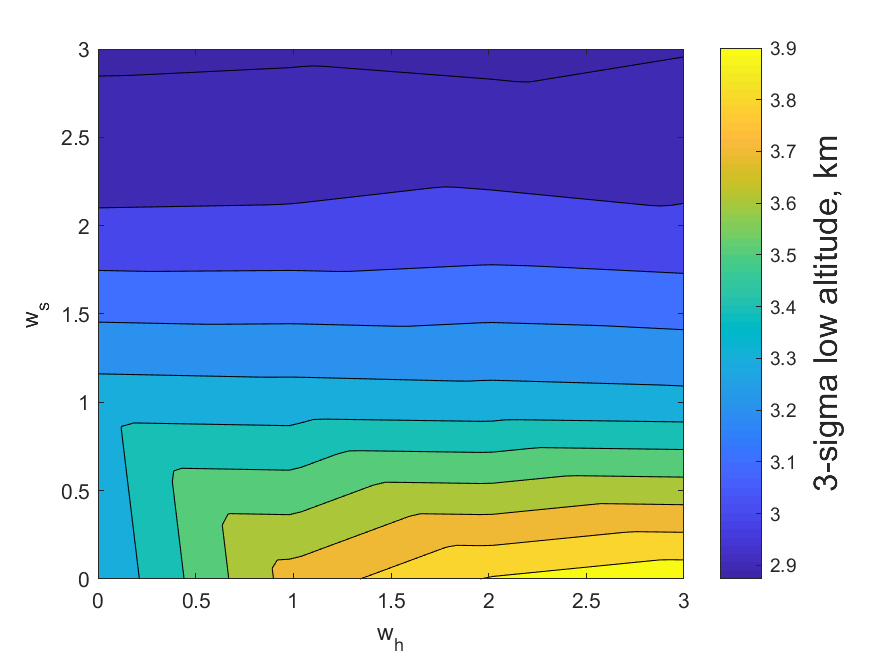
\includegraphics[width=0.75\textwidth]{ddp/matlab/ClosedLoopAltitude}
	\caption{Contours of the unscented transform estimated 3$\sigma$ low altitude for different weights. As one should expect, this quantity is maximized for $w_h=3,\,w_0$, and drops as the weight on range errors increases. Red circles indicate the weights for which the optimal control problem was solved.}
	\label{fig_weight_sweep_altitude}
\end{figure}
\begin{figure}[h!]
	\centering
	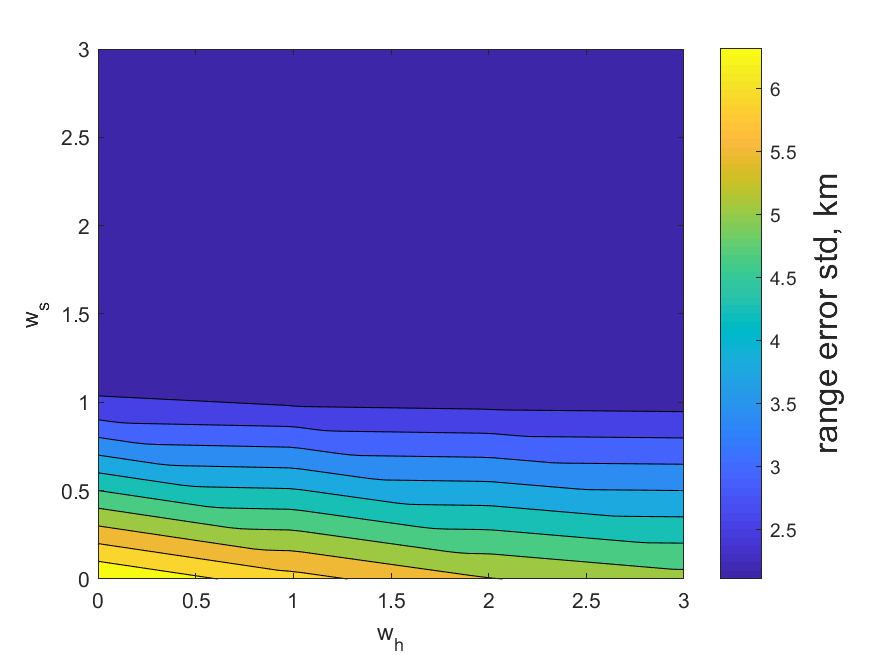
\includegraphics[width=0.75\textwidth]{ddp/matlab/ClosedLoopRangeError}
	\caption{Contours of the unscented transform estimated downrange standard deviation. Range error rapidly improves as $w_s$ is raised to 1, and diminishing returns occur for larger values. Red circles indicate the weights for which the optimal control problem was solved.}
	\label{fig_weight_sweep_dr}
\end{figure}
%\begin{figure}[h!]
%	\centering
%	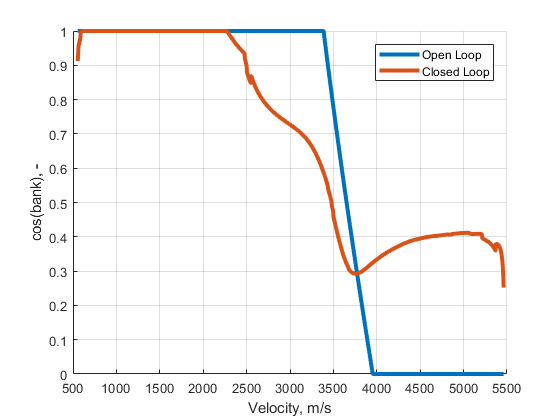
\includegraphics[width=1\textwidth]{ddp/control}
%	\caption{Both solutions display a lower lift segment at high velocities before transitioning to a full lift up arc until the terminal velocity is reached. The primary difference is the closed-loop control leaves substantial margin for feedback control early on until the trajectory errors have been reduced. Once parametric uncertainty is introduced, margin is expected to be required throughout the trajectory.}
%\end{figure}
This also highlights the power of the approach as a design tool. If, for example, the $3\sigma$-low terminal altitude is not sufficient for any values of $w_h,\,w_s$, then some aspect of the mission must be reconsidered: increase the terminal velocity, increase the vehicle $L/D$, decrease ballistic coefficient, etc. If a $3\sigma$-low altitude limit is known, then only points corresponding to those meeting this limit are considered, and the point with the lowest downrange error may be selected. 

\subsection*{Reference Trajectory Comparison}
Having demonstrated the potential benefits of weighting the terminal standard deviations, we proceed to further demonstrate the superiority of design under uncertainty over heuristically chosen fixed bank angle margins.
In this section we compare the results of closed-loop optimization under uncertainty with deterministic trajectory design methods that do not explicitly account for uncertainty. Scenario 1 employs the proposed method with $w_h=1, w_s=1$ to design a robust reference trajectory. Scenarios 2-4 solve a deterministic optimal control problem that maximizes terminal altitude subject to different bank angle limits in order to preserve different amounts of margin. The four scenarios are summarized in Table~\ref{table_comparison}. Figure~\ref{fig_control_comparison} shows the resulting control profiles for the four scenarios.

Scenario 2 is the altitude optimal case with no margin, and thus is has the highest mean altitude. However, the lack of margin causes poor performance in dispersed trajectories, leading to the lowest $ 3\sigma $ low altitude and the largest range errors.As the amount of margin is heuristically increased at all velocities, the range error drops, as does the altitude variance. However, the $ 3\sigma $-low altitude displays non-monotonic behavior because the increased margin is also lowering the mean altitude in exchange for robustness; this is why scenario 3 has a higher low altitude than scenario 4. Finally, scenario 1 achieves simultaneously the highest $ 3\sigma$-low altitude and the lowest range error. This demonstrates the ability of optimal control under uncertainty to design robust trajectories. Additionally, the flexibility of the weights allows the trajectory designer to trade between range errors and altitude freely, to the extent that covariance shaping techniques can alter closed-loop performance. This is the subject of the following section. Figures~\ref{fig_robust_alt}-\ref{fig_robust_range} show the estimated $3\sigma$ deviations around the mean as well as the sigma point trajectories for scenario 1.
\begin{figure}[h!]
	\centering
	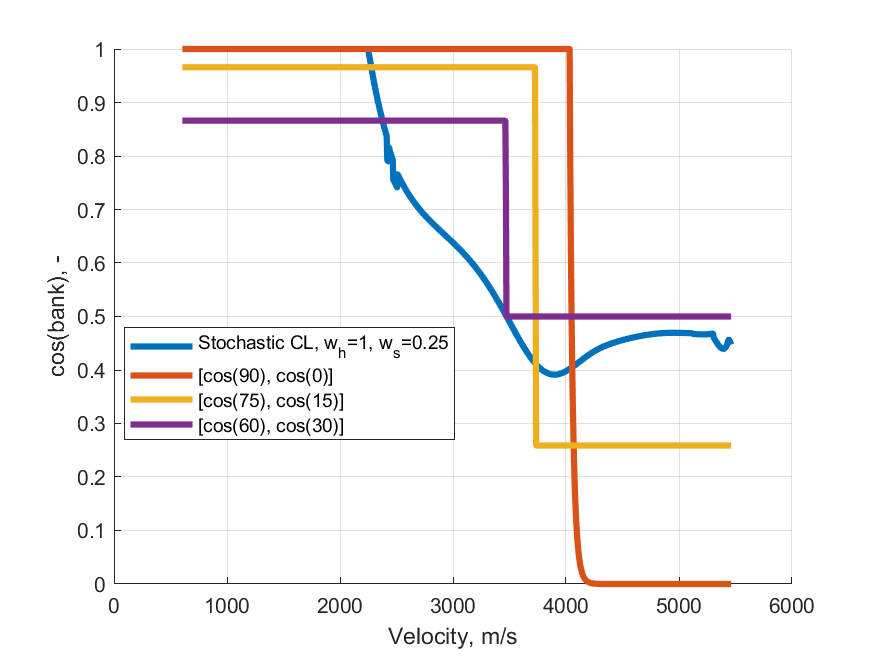
\includegraphics[width=1\textwidth]{ddp/matlab/ComparisonControl}
	\caption{The profiles from deterministic optimal control exhibit the well known bang-bang structure of altitude optimal trajectories. In comparison, the robust trajectory saturates from 4000 m/s to 3000 m/s but preserves margin at lower velocities.}
	\label{fig_control_comparison}
\end{figure}
\begin{table}[h!]
	\centering
	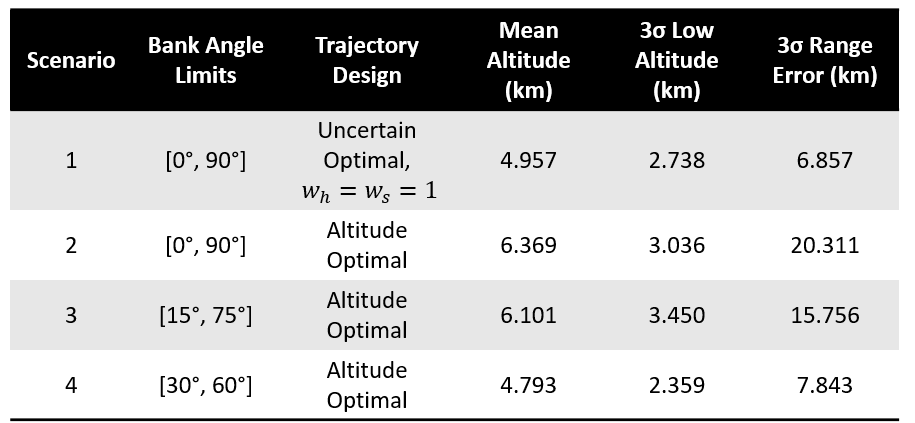
\includegraphics[width=1\textwidth]{ddp/comparison_table}
	\caption{The robust trajectory designed with knowledge of the problem uncertainty outperforms heuristically designed reference trajectories in $3\sigma$ low altitude and range errors.}
	\label{table_comparison}
\end{table}
\begin{figure}[h!]
	\centering
	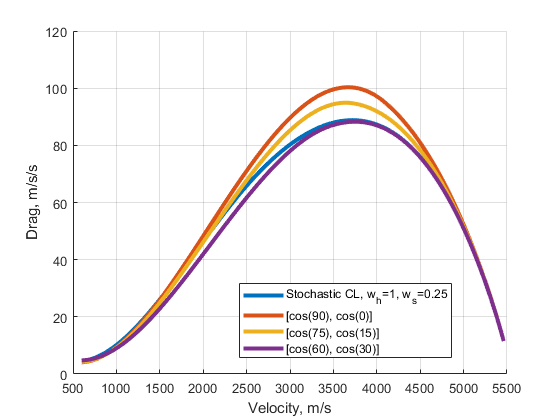
\includegraphics[width=1\textwidth]{ddp/matlab/ComparisonDrag}
	\caption{Reference drag profile for each of the four scenarios in Table~\ref{table_comparison}.}
	\label{fig_drag}
\end{figure}
\begin{figure}[h!]
	\centering
	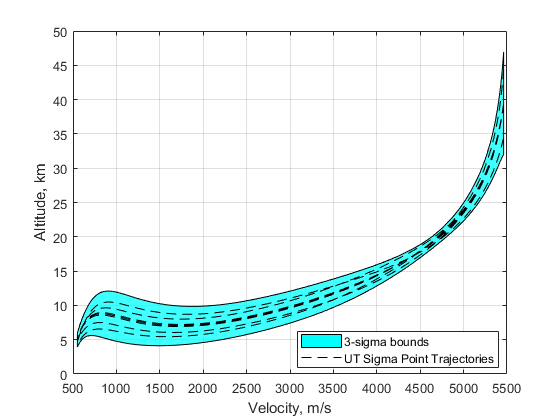
\includegraphics[width=1\textwidth]{ddp/matlab/RobustTrajAlt}
	\caption{Dispersed altitude performance for scenario 1.}
	\label{fig_robust_alt}
\end{figure}
\begin{figure}[h!]
	\centering
	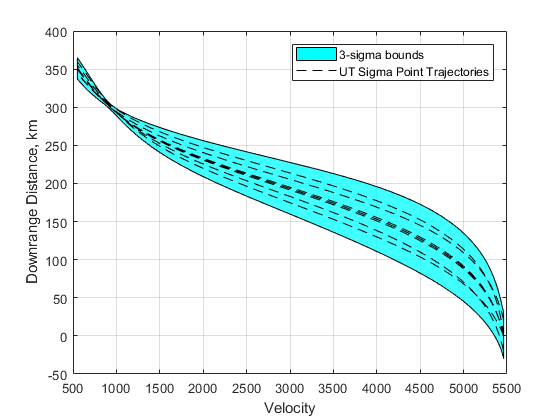
\includegraphics[width=1\textwidth]{ddp/matlab/RobustTrajRange}
	\caption{Dispersed range performance for scenario 1.}
	\label{fig_robust_range}
\end{figure}


%\subsection{open-loop vs closed-loop}
%The problem is solved with the weights $w_h = 0.001$, $w_s = 0.01$ and assuming the initial state covariance $\cov = \mathrm{diag}([2500^2,0.25^2,1000^2])$. In the closed-loop scenario, drag, flight path angle, and range-to-go are the feedback states, and the feedback gains are constants $[0.1, -50, 0.1]$. 
%
%\begin{figure}[h!]
%	\centering
%	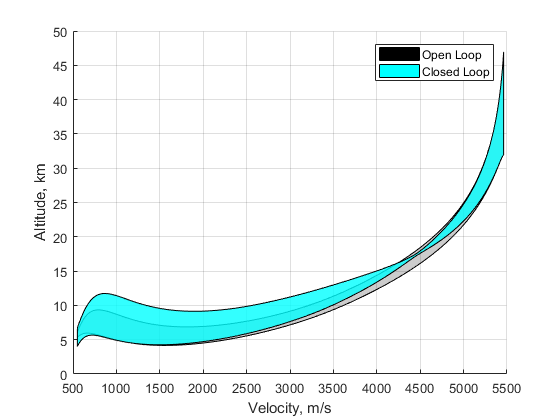
\includegraphics[width=1\textwidth]{ddp/altitude}
%	\caption{The mean altitude remains high but the controller induces additional altitude variance in order to track the downrange distance.}
%	\label{fig_alt}
%\end{figure}
%\begin{figure}[h!]
%	\centering
%	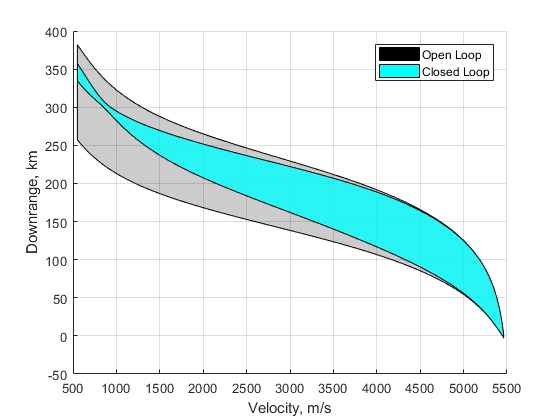
\includegraphics[width=1\textwidth]{ddp/downrange}
%	\caption{The controller produces a substantial reduction in downrange error at a small increase to altitude variance.}
%	\label{fig_dr}
%\end{figure}
%\begin{figure}[h!]
%	\centering
%	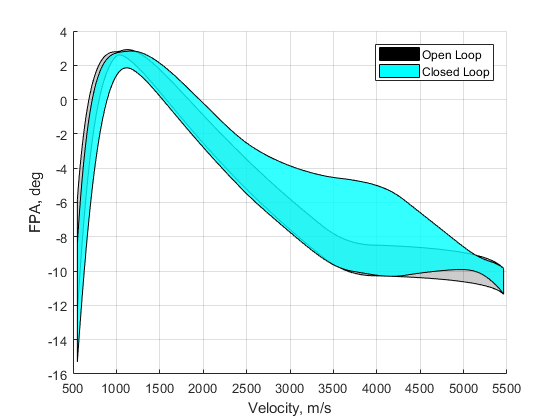
\includegraphics[width=1\textwidth]{ddp/fpa}
%	\caption{Worth noting is the non-monotonicity of the flight path angle variance, which increases substantially during the closed-loop control. The nonlinearity of the trajectory is used to achieve reduced terminal variance in the other state variables.}
%	\label{fig_fpa}
%\end{figure}
%\begin{figure}[h!]
%	\centering
%	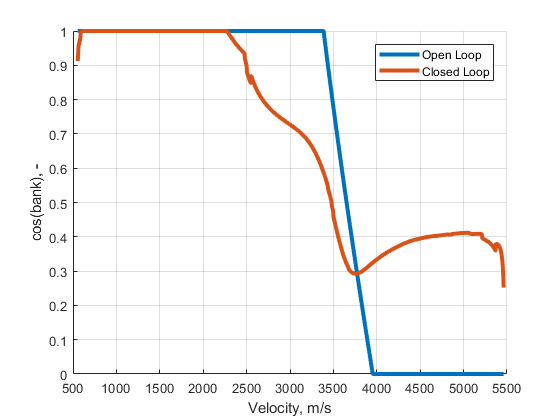
\includegraphics[width=1\textwidth]{ddp/control}
%	\caption{Both solutions display a lower lift segment at high velocities before transitioning to a full lift up arc until the terminal velocity is reached. The primary difference is the closed-loop control leaves substantial margin for feedback control early on until the trajectory errors have been reduced. Once parametric uncertainty is introduced, margin is expected to be required throughout the trajectory.}
%	\label{fig_control}
%\end{figure}

%\subsection{Equal Weight Comparison}
%% Data saved in EqualWeightComparison.mat
%Compare scenarios with the same weights: open-loop, CL with fixed gains, CL with optimized gains. Also add results for flying the open-loop profile but with either/both the fixed gains or the optimized gains. Show that both sets of gains improve the results of course, but the optimized gains are only "optimal" in conjunction with the reference profile - synergy between the two improves the net result.


%\subsection{Monte Carlo Validation}
%There two objectives of this section are
%\begin{enumerate}
%\item Verify that the mean and variances computed via Unscented Transform are sufficiently close to MC results
%\item Check that mean and std are an applicable description of the terminal distributions by examining skew and kurtosis
%\end{enumerate}
%Sweep across $ w_s $ with $w_h=1$ fixed, and find the point (in terminal std deviation of range) where the UT approximation breaks down

%\subsection*{LQR and Apollo Gains}
%In this section we investigate the impact of time-varying gains computed via LQR, or using the state of the art modified Apollo gains. 

%\subsection*{Discussion}
%The second order method consistently finds the same solution for open-loop and closed-loop when the gains are not optimization variables. When the gains are also optimized, the initial guess has a large effect on the solution found, suggesting a difficult optimization landscape with many local minima. 

\section*{Conclusion}
We have presented a new approach to generating robust, altitude optimal reference trajectories for Mars entry guidance. The entry guidance problem is posed as an optimal control problem with uncertain initial state and parameters. The statistics required to evaluate the objective function are estimated with sample trajectories computed via the unscented transform. Differential dynamic programming is demonstrated to be an effective way to solve the resulting large-scale optimal control problem. By weighting the altitude optimization objective with standard deviations on altitude and downrange distance, entry trajectories robust to the modeled uncertainties are generated. Monte Carlo simulations were conducted to verify the improvement over conventional design techniques based on deterministic optimal control. 
%\bibliographystyle{AAS_publication}
\bibliography{bib}

\end{document}